\chapter{Additional Plots and Parameters\label{chap:plus_plots_params}}

\section{Plots}
\label{sec:plus_plots}

\subsection{Interaction Consisency Plots}
\label{sec:intercons}
\begin{figure}[H]
  \centering
  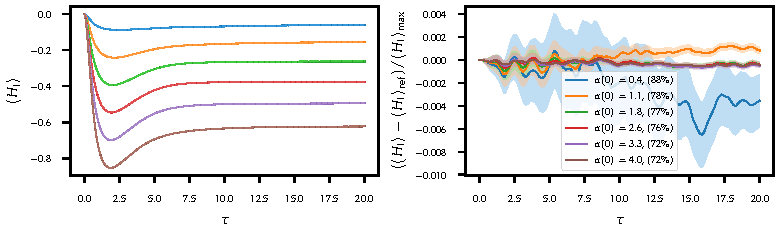
\includegraphics{figs/one_bath_syst/delta_interaction_consistency}
  \caption{\label{fig:delta_interaction_consistency}Interaction
    consistency plot for \cref{sec:one_bathcoup_strength}, similar to
    \cref{fig:stocproc_systematics}.}
\end{figure}

\subsection{More Plots for Single Bath Modulation}
\label{sec:extra_single_plots}
\begin{figure}[H]
  \centering
  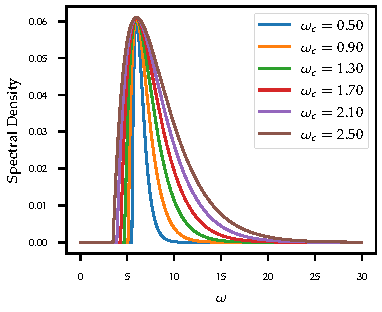
\includegraphics{figs/one_bath_mod/omega_sd_weak}
  \caption{\label{fig:omega_couplings_weak} Similar
    to \cref{fig:omega_couplings_and_energies} but for weaker coupling.}
\end{figure}

\begin{figure}[H]
  \centering
  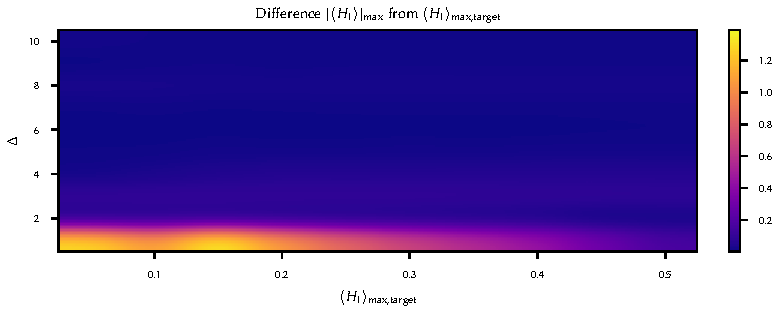
\includegraphics{figs/one_bath_mod/interaction_tuning_success}
  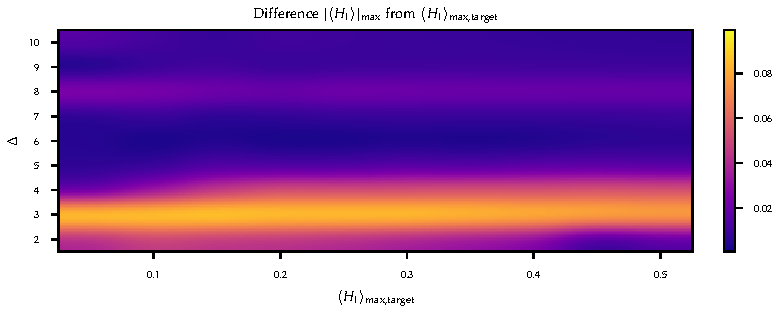
\includegraphics{figs/one_bath_mod/interaction_tuning_success_detail}
  \caption{\label{fig:interaction_tuning_success} The relative
    difference of the peak interaction energies from the target
    (\(0.4\)). The case of \(Δ=1\) appears to be the least reliable
    with deviation of more than \(100\%\) for lower target values. The
  lower panel shows the same situation excluding the \(Δ=1\) case.}
\end{figure}


\subsection{More Plots for the Otto Cycle}
\label{sec:otto_plots}
\begin{figure}[H]
  \centering
  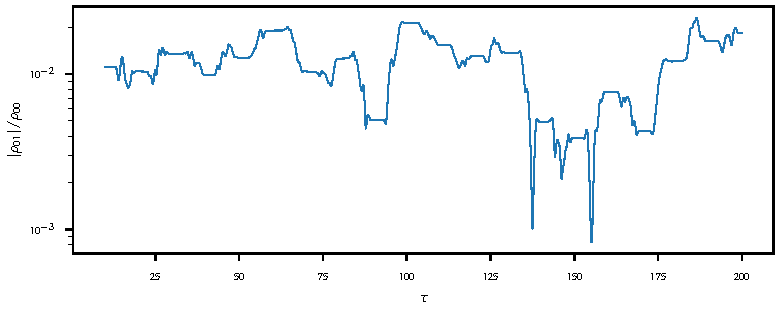
\includegraphics{figs/otto/coherences}
  \caption{\label{eq:otto_coherences} The coherences of the system
    state of the otto cycle in \cref{sec:otto}.}
\end{figure}
\begin{figure}[H]
  \centering
  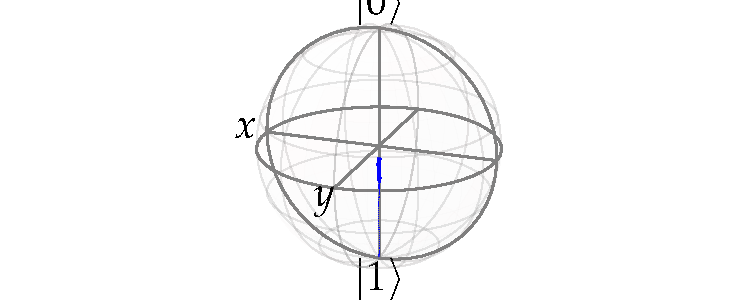
\includegraphics{figs/otto/bloch}
  \caption{\label{eq:otto_bloch} The system state of the model
    \cref{sec:otto} in the bloch sphere.}
\end{figure}

\section{Parameters}
\label{sec:plus_params}
\subsection{Modulation with a single Bath}
\label{sec:plus_mod_single}

\begin{table}[H]
  \centering
  \begin{tabular}{lll}
    \hline
    $ω_c$              & $2$     & $2$    \\
    $α(0)$             & $0.7$   & $0.7$  \\
    $T$                & $5$     & $5$    \\
    $N$                & $10000$ & $2000$ \\
    $k_{\mathrm{max}}$ & $5$     & $5$    \\
    \hline
  \end{tabular}
  \caption{\label{tab:plus_friction}Additional parameters for
    \cref{fig:quant_frict}.}
\end{table}


\begin{table}[H]
  \centering
  \begin{tabular}{lll}
    \hline
    $ω_c$              & $2$    & $2$    \\
    $α(0)$             & $0.7$  & $0.7$  \\
    $T$                & $5$    & $5$    \\
    $N$                & $1000$ & $1000$ \\
    $k_{\mathrm{max}}$ & $5$    & $5$    \\
    \hline
  \end{tabular}
  \caption{\label{tab:plus_system}Additional parameters for
    \cref{fig:quant_frict_sys_no_sys}.}
\end{table}

\begin{table}[H]
  \centering
  \begin{tabular}{lllllll}
    \hline
    $ω_c$              & $0.50$     & $0.90$     & $1.30$     & $1.70$     & $2.10$     & $2.50$     \\
    $α(0)$             & $1.32$     & $1.42$     & $1.44$     & $1.33$     & $1.25$     & $1.37$     \\
    $T$                & $5.00$     & $5.00$     & $5.00$     & $5.00$     & $5.00$     & $5.00$     \\
    $N$                & $10000.00$ & $10000.00$ & $10000.00$ & $10000.00$ & $10000.00$ & $10000.00$ \\
    $k_{\mathrm{max}}$ & $5.00$     & $5.00$     & $5.00$     & $5.00$     & $5.00$     & $5.00$     \\
    BCF Terms          & $7.00$     & $7.00$     & $7.00$     & $7.00$     & $7.00$     & $7.00$     \\
    \hline
  \end{tabular}

  \caption{\label{tab:plus_omega}Additional parameters for the models in
     \cref{sec:extr_mem}.}
\end{table}

\begin{longtable}[c]{lllllll}
  \toprule
   $ω_c$   & $ω_s$   & $α(0)$   & $T$    & $N$       & $k_{\mathrm{max}}$   & BCF Terms   \\
  \midrule
   $1.00$  & $1.00$  & $0.88$   & $5.00$ & $2000.00$ & $6.00$
                                                                            & $7.00$      \\
  \bottomrule
  \caption{\label{tab:plus_mod_en}Additional parameters for the models in
     \cref{sec:speedlim} for the interaction energy optimized case. We
  have omitted all but the first row.}
\end{longtable}


\begin{table}[H]
  \centering
  \begin{tabular}{lllllll}
  \toprule
   $ω_c$   & $ω_s$   & $α(0)$   & $T$    & $N$       & $k_{\mathrm{max}}$   & BCF Terms   \\
  \midrule
   $1.00$  & $4.50$  & $0.78$   & $5.00$ & $2000.00$ & $7.00$
                                                                            & $7.00$      \\
  \bottomrule
  \end{tabular}
  \caption{\label{tab:plus_tune}Additional parameters for the models
    in \cref{sec:modcoup_reso}.  We have omitted all but the first
    row.}
\end{table}
